%CS-113 S18 HW-2
%Released: 2-Feb-2018
%Deadline: 16-Feb-2018 7.00 pm
%Authors: Abdullah Zafar, Emad bin Abid, Moonis Rashid, Abdul Rafay Mehboob, Waqar Saleem.


\documentclass[addpoints]{exam}

% Header and footer.
\pagestyle{headandfoot}
\runningheadrule
\runningfootrule
\runningheader{CS 113 Discrete Mathematics}{Homework II}{Spring 2018}
\runningfooter{}{Page \thepage\ of \numpages}{}
\firstpageheader{}{}{}

\boxedpoints
\printanswers
\usepackage[table]{xcolor}
\usepackage{amsfonts,graphicx,amsmath,hyperref}
\title{Habib University\\CS-113 Discrete Mathematics\\Spring 2018\\HW 2}
\author{$si03481$}  % replace with your ID, e.g. oy02945
\date{Due: 19h, 16th February, 2018}


\begin{document}
\maketitle

\begin{questions}



\question

%Short Questions (25)

\begin{parts}

  
  \part[5] Determine the domain, codomain and set of values for the following function to be 1) partial and 2) total: 
  \begin{center}
    $y=\sqrt{x}$
  \end{center}

  \begin{solution}
    % Write your solution here
    The function does not map all values of the domain, these include the negative integers. Therefore the function is partial for the domain of all integers and the codomain of all real numbers.
    \newline
    As all the values of the domain are mapped to some values of the codomain when the domain is of all positive integers and the codomain is of all real numbers, therefore it is a total function.
  \end{solution}
  
  \part[5] Explain whether $f$ is a function from the set of all bit strings to the set of integers if $f(S)$ is the smallest $i \in \mathbb{Z}$� such that the $i$th bit of S is 1 and $f(S) = 0$ when S is the empty string. 
  
  \begin{solution}
    % Write your solution here
    \newline
    The bit strings which are only of 0's does not have 1's in them thus the relation is not a function but is characterized as a partial function.
  \end{solution}

  \part[15] For $X,Y \in S$, explain why (or why not) the following define an equivalence relation on $S$:
  \begin{subparts}
    \subpart ``$X$ and $Y$ have been in class together"
    \subpart ``$X$ and $Y$ rhyme"
    \subpart ``$X$ is a subset of $Y$"
  \end{subparts}

  \begin{solution}
    % Write your solution here
    \newline
    i). ``$X$ and $Y$ have been in class together"
    \newline
    Since it can be said that X is in class together with X itself thus the statement follows a Reflexive relation. As the statement that X is in class with Y also results to the inverse relation that Y is in class with X, therefore the statement also follows a Symmetric relation. X and Y have been in class together and Y and Z have been in class together does not means that X and Z have been in class together if multiple classes are taken into consideration, therefore the statement does not follows a transitive relation. Hence it can be said that the statement does not have an equivalence relation.
    \newline
    \newline
    ii). ``$X$ and $Y$ rhyme"
    \newline
    X definitely rhymes with itself thus the statement follows a Reflexive relation.
    If X rhymes with Y then Y also rhymes with X and therefore the statement follows a symmetric relation as well. If X rhymes with Y and Y rhymes with Z then it also means that X rhymes with Z therefore the statement also follows a transitive relation and hence have an equivalence relation.
    \newline
    \newline
    iii). ``$X$ is a subset of $Y$"
    \newline
    Every set is a subset of itself therefore the statement automatically follows a Reflexive relation. If X is a subset of Y and Y is a subset of Z, this means that Z is the largest set which encompasses X and Y and therefore X is also a subset of Z which means the statement also follows a Transitive relation. If X is a subset of Y, this means that X is the smaller set and Y cannot be a subset of X. Therefore the statement does not follows a Symmetric relation and hence does not have an equivalence relation. 
    \newline
    
  \end{solution}

\end{parts}

%Long questions (75)
\question[15] Let $A = f^{-1}(B)$. Prove that $f(A) \subseteq B$.
  \begin{solution}
    % Write your solution here
    \newline
    For two elements in the set A and B, that are a1 and b1. The relationship $a1=f^{-1}(b1)$ and $b1= f(a1)$ can be proved since $f(f^{-1}(b1))=b1$ hence $f(i)=f(f^{-1}(j))$ is equivalent to $f(a1)=b1$. Since $b1=f(a1) \in B$ meaning $b1=f(a1)\subseteq B$. This property will be true for all the elements in A and B therefore it can be said $f(A)\subseteq B$ 
  \end{solution}

\question[15] Consider $[n] = \{1,2,3,...,n\}$ where $n \in \mathbb{N}$. Let $A$ be the set of subsets of $[n]$ that have even size, and let $B$ be the set of subsets of $[n]$ that have odd size. Establish a bijection from $A$ to $B$, thereby proving $|A| = |B|$. (Such a bijection is suggested below for $n = 3$) 

\begin{center}

  \begin{tabular}{ |c || c | c | c |c |}
    \hline
 A & $\emptyset$ & $\{2,3\}$ & $\{1,3\}$ & $\{1,2\}$ \\ \hline
 B & $\{3\}$ & $\{2\}$ & $\{1\}$ & $\{1,2,3\}$\\\hline
\end{tabular}
\end{center}

  \begin{solution}
    % Write your solution here
    \newline
    To prove a bijection we need to prove that an injective and both a surjective relation is being followed.
    \newline
    To prove the injective property, let $A_1$ and $A_2$ be two subsets and consider $f(A_1)=f(A_2)$. Either we have 
    \newline
    $A_1 - \{n\} = f(A_1)=f(A_2)=A_2-\{n\}$
    \newline
    or
    \newline
    $A_1 \cup \{n\}= f(A_1)=f(A_2)=A_2 \cup \{n\}$
    \newline
    In either of the cases we can conclude that $A_1=A_2$, and so it is injective.
    \newline
    To prove the surjective relation, let B be an element of the range f (i.e a subset of odd size). If B contains n, then B -$\{n\}$ is a subset of even size that maps to B under f. If B does not contain n, then B $\cup \{n\}$ is a subset of even size that maps to B under f. 
    \newline
    Since everything in the image has something in the domain that maps to it, f is surjective.
    \newline
    Since it follows an injective and surjective relation, we can establish a bijection from A to B.
    
  \end{solution}
  
\question Mushrooms play a vital role in the biosphere of our planet. They also have recreational uses, such as in understanding the mathematical series below. A mushroom number, $M_n$, is a figurate number that can be represented in the form of a mushroom shaped grid of points, such that the number of points is the mushroom number. A mushroom consists of a stem and cap, while its height is the combined height of the two parts. Here is $M_5=23$:

\begin{figure}[h]
  \centering
  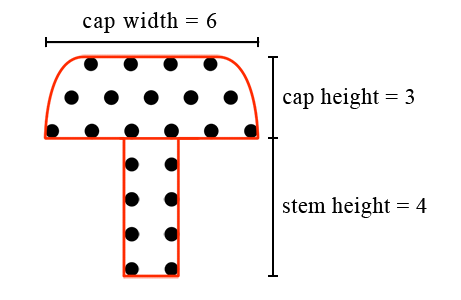
\includegraphics[scale=1.0]{m5_figurate.png}
  \caption{Representation of $M_5$ mushroom}
  \label{fig:mushroom_anatomy}
\end{figure}

We can draw the mushroom that represents $M_{n+1}$ recursively, for $n \geq 1$:
\[ 
    M_{n+1}=
    \begin{cases} 
      (\textrm{Cap\_width}(M_n) + 1) + (\textrm{Stem\_height}(M_n) + 1) + \textrm{Cap\_height}(M_n)  & n \textrm{ is even} \\
      (\textrm{Cap\_width}(M_n) + 1) + (\textrm{Stem\_height}(M_n) + 1)  + (\textrm{Cap\_height}(M_n)+1) & n \textrm{ is odd}  \\      
   \end{cases}
\]

Study the first five mushrooms carefully and make sure you can draw subsequent ones using the recurrence above.

\begin{figure}[h]
  \centering
  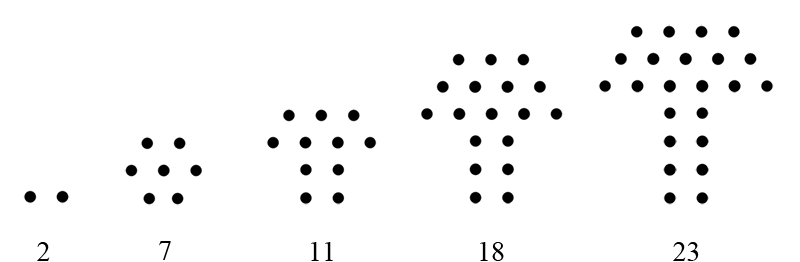
\includegraphics{mushroom_series.png}
  \caption{Representation of $M_1,M_2,M_3,M_4,M_5$ mushrooms}
  \label{fig:mushroom_anatomy}
\end{figure}

  \begin{parts}
    \part[15] Derive a closed-form for $M_n$ in terms of $n$.
  \begin{solution}
    % Write your solution here
    \newline
    For n=1
    \newline
    Stem\_height(0)
    \newline
    n=2
    \newline
    Stem\_height(1)
    \newline
    n=3
    \newline
    Stem\_height(2)
    \newline
    n=4
    \newline
    Stem\_height(3)
    \newline
    n=5
    \newline
    Stem\_height(4)
    \newline
    Therefore the general formula for Stem height is Stem\_height(n-1)
    \newline
    The generic formula for the dots in Stem height will be = 2(n-1)
    \newline
    \newline
    For n=1
    \newline
    Cap\_width(2)
    \newline
    n=2
    \newline
    Cap\_width(3)
    \newline
    n=3
    \newline
    Cap\_width(4)
    \newline
    n=4
    \newline
    Cap\_width(5)
    \newline
    n=5
    \newline
    Cap\_width(6)
    \newline
    Therefore the general formula for Cap width is Cap\_width(n+1) and so is the generic formula for the dots of Cap width.
    \newline
    \newline
    For n=1
    \newline
    Cap\_height(1)
    \newline
    n=2
    \newline
    Cap\_height(2)
    \newline
    n=3
    \newline
    Cap\_height(2)
    \newline
    n=4
    \newline
    Cap\_height(3)
    \newline
    n=5
    \newline
    Cap\_height(3)
    $\newline$
    Therefore the general formula for Cap height turns out to be Cap\_height($\dfrac{3+2n+(-1)^n}{4}$) as for example when n=4, Cap\_height($\dfrac{3+2(4)+(-1)^4}{4}$) = 3
    \newline and when n=5, Cap\_height($\dfrac{3+2(5)+(-1)^5}{4}$) = 3 
    \newline
    This also results to $|\dfrac{n}{2}|+1$
    \newline
    The generic formula for the dots in Cap Height can be computized to $|\dfrac{n}{2}|+1-\dfrac{|\dfrac{n}{2}|(|\dfrac{n}{2}|+1)}{2}$
    \newline
    The Generic Formula for the dots in whole mushroom is the (number of dots in cap width)(number of dots in cap height)+number of dots in stem height.
    \newline
    \newline
    $M_n = (n+1)(|\dfrac{n}{2}|+1-\dfrac{|\dfrac{n}{2}|(|\dfrac{n}{2}|+1)}{2})+2(n-1)$
    \newline
    
  \end{solution}
    \part[5] What is the total height of the $20$th mushroom in the series? 
  \begin{solution}
    % Write your solution here
    Total Height = Stem Height + Cap Height
    \newline
    Total Height = Stem\_height(20-1) + Cap\_height($\dfrac{3+2(20)+(-1)^{20}}{4}$)
    \newline
    Total Height = 19 + 11
    \newline
    Total Height = 30
  \end{solution}
\end{parts}

\question
    The \href{https://en.wikipedia.org/wiki/Fibonacci_number}{Fibonacci series} is an infinite sequence of integers, starting with $1$ and $2$ and defined recursively after that, for the $n$th term in the array, as $F(n) = F(n-1) + F(n-2)$. In this problem, we will count an interesting set derived from the Fibonacci recurrence.
    
The \href{http://www.maths.surrey.ac.uk/hosted-sites/R.Knott/Fibonacci/fibGen.html#section6.2}{Wythoff array} is an infinite 2D-array of integers where the $n$th row is formed from the Fibonnaci recurrence using starting numbers $n$ and $\left \lfloor{\phi\cdot (n+1)}\right \rfloor$ where $n \in \mathbb{N}$ and $\phi$ is the \href{https://en.wikipedia.org/wiki/Golden_ratio}{golden ratio} $1.618$ (3 sf).

\begin{center}
\begin{tabular}{c c c c c c c c}
 \cellcolor{blue!25}1 & 2 & 3 & 5 & 8 & 13 & 21 & $\cdots$\\
 4 & \cellcolor{blue!25}7 & 11 & 18 & 29 & 47 & 76 & $\cdots$\\
 6 & 10 & \cellcolor{blue!25}16 & 26 & 42 & 68 & 110 & $\cdots$\\
 9 & 15 & 24 & \cellcolor{blue!25}39 & 63 & 102 & 165 & $\cdots$ \\
 12 & 20 & 32 & 52 & \cellcolor{blue!25}84 & 136 & 220 & $\cdots$ \\
 14 & 23 & 37 & 60 & 97 & \cellcolor{blue!25}157 & 254 & $\cdots$\\
 17 & 28 & 45 & 73 & 118 & 191 & \cellcolor{blue!25}309 & $\cdots$\\
 $\vdots$ & $\vdots$ & $\vdots$ & $\vdots$ & $\vdots$ & $\vdots$ & $\vdots$ & \color{blue}$\ddots$\\
 

\end{tabular}
\end{center}

\begin{parts}
  \part[10] To begin, prove that the Fibonacci series is countable.
 
    \begin{solution}
    % Write your solution here
    \newline
    For any series to be countable it has to form bijection mapping with a subset of natural numbers. Now to form a fibonacci sequence. For every natural number if the golden ratio is applied to it, it will converge to a number. This proves that it is bijective as all the domain is mapped to a certain codomain and all the codomain is mapped to a certain number too.
    
  \end{solution}
  \part[15] Consider the Modified Wythoff as any array derived from the original, where each entry of the leading diagonal (marked in blue) of the original 2D-Array is replaced with an integer that does not occur in that row. Prove that the Wythoff Array is countable. 

  \begin{solution}
    % Write your solution here
    Every row of the wythoff series is a modified fibonacci series, since we have proven that the fibonacci sereis is countable every row must also be unique and countable
    every element can thus be described with a unique coordinate. each coordinate will correspond to a unique elemenet and each elemtn 
  \end{solution}
\end{parts}

\end{questions}

\end{document}
